\documentclass{article}

% Bibliography
\usepackage{natbib}
\bibpunct{(}{)}{;}{a}{}{;}

% Use 'It was found that A is B (Name 1234)' style
\setcitestyle{authoryear,open={},close={}}

% Affiliations
\usepackage{authblk}
\title{Stage 1 Registered Report: The error when inferring phylogenies with incipient species by a Birth-Death model}
% \subtitle{Should protracted speciation be incorporated in phylogenetic tree construction methods?}

\author[1]{Rich\`el J.C. Bilderbeek}
\author[1]{Rampal S. Etienne}
\affil[1]{Groningen Institute for Evolutionary Life Sciences, University of Groningen, Groningen, The Netherlands}

% Load my functions
% The functions used

% My first function, kept for nostalic reasons
\newcommand{\sayhello}{hello and howdy!}

% Making a note
\newcommand\note[1]{\textcolor{green}{\todo{#1}}}

% From https://tex.stackexchange.com/a/98034
\newcommand*\mean[1]{\overline{#1}}

% From https://tex.stackexchange.com/a/101138
% \newcommand\reallywidetilde[1]{\ThisStyle{%
%   \setbox0=\hbox{$\SavedStyle#1$}%
%   \stackengine{-.1\LMpt}{$\SavedStyle#1$}{%
%     \stretchto{\scaleto{\SavedStyle\mkern.2mu\AC}{.5150\wd0}}{.6\ht0}%
%   }{O}{c}{F}{T}{S}%
% }}

% Adapted from 'mean', use 'reallywidetilde'
% \newcommand*\median[1]{\reallywidetilde{#1}}

\newcommand*\median[1]{\widetilde{#1}}

%%%%%%%%%%%%%%%%%%%%%%%%%%%%%%%%%%%%%%%%%%%%%%%%%%%%%%%%%%%%%%%%%%%%%%%%%%%%%%%%
% Create the TikZ picture for fig:experiment
%%%%%%%%%%%%%%%%%%%%%%%%%%%%%%%%%%%%%%%%%%%%%%%%%%%%%%%%%%%%%%%%%%%%%%%%%%%%%%%%
\newcommand{\CreateTikzFigureExperiment} {

  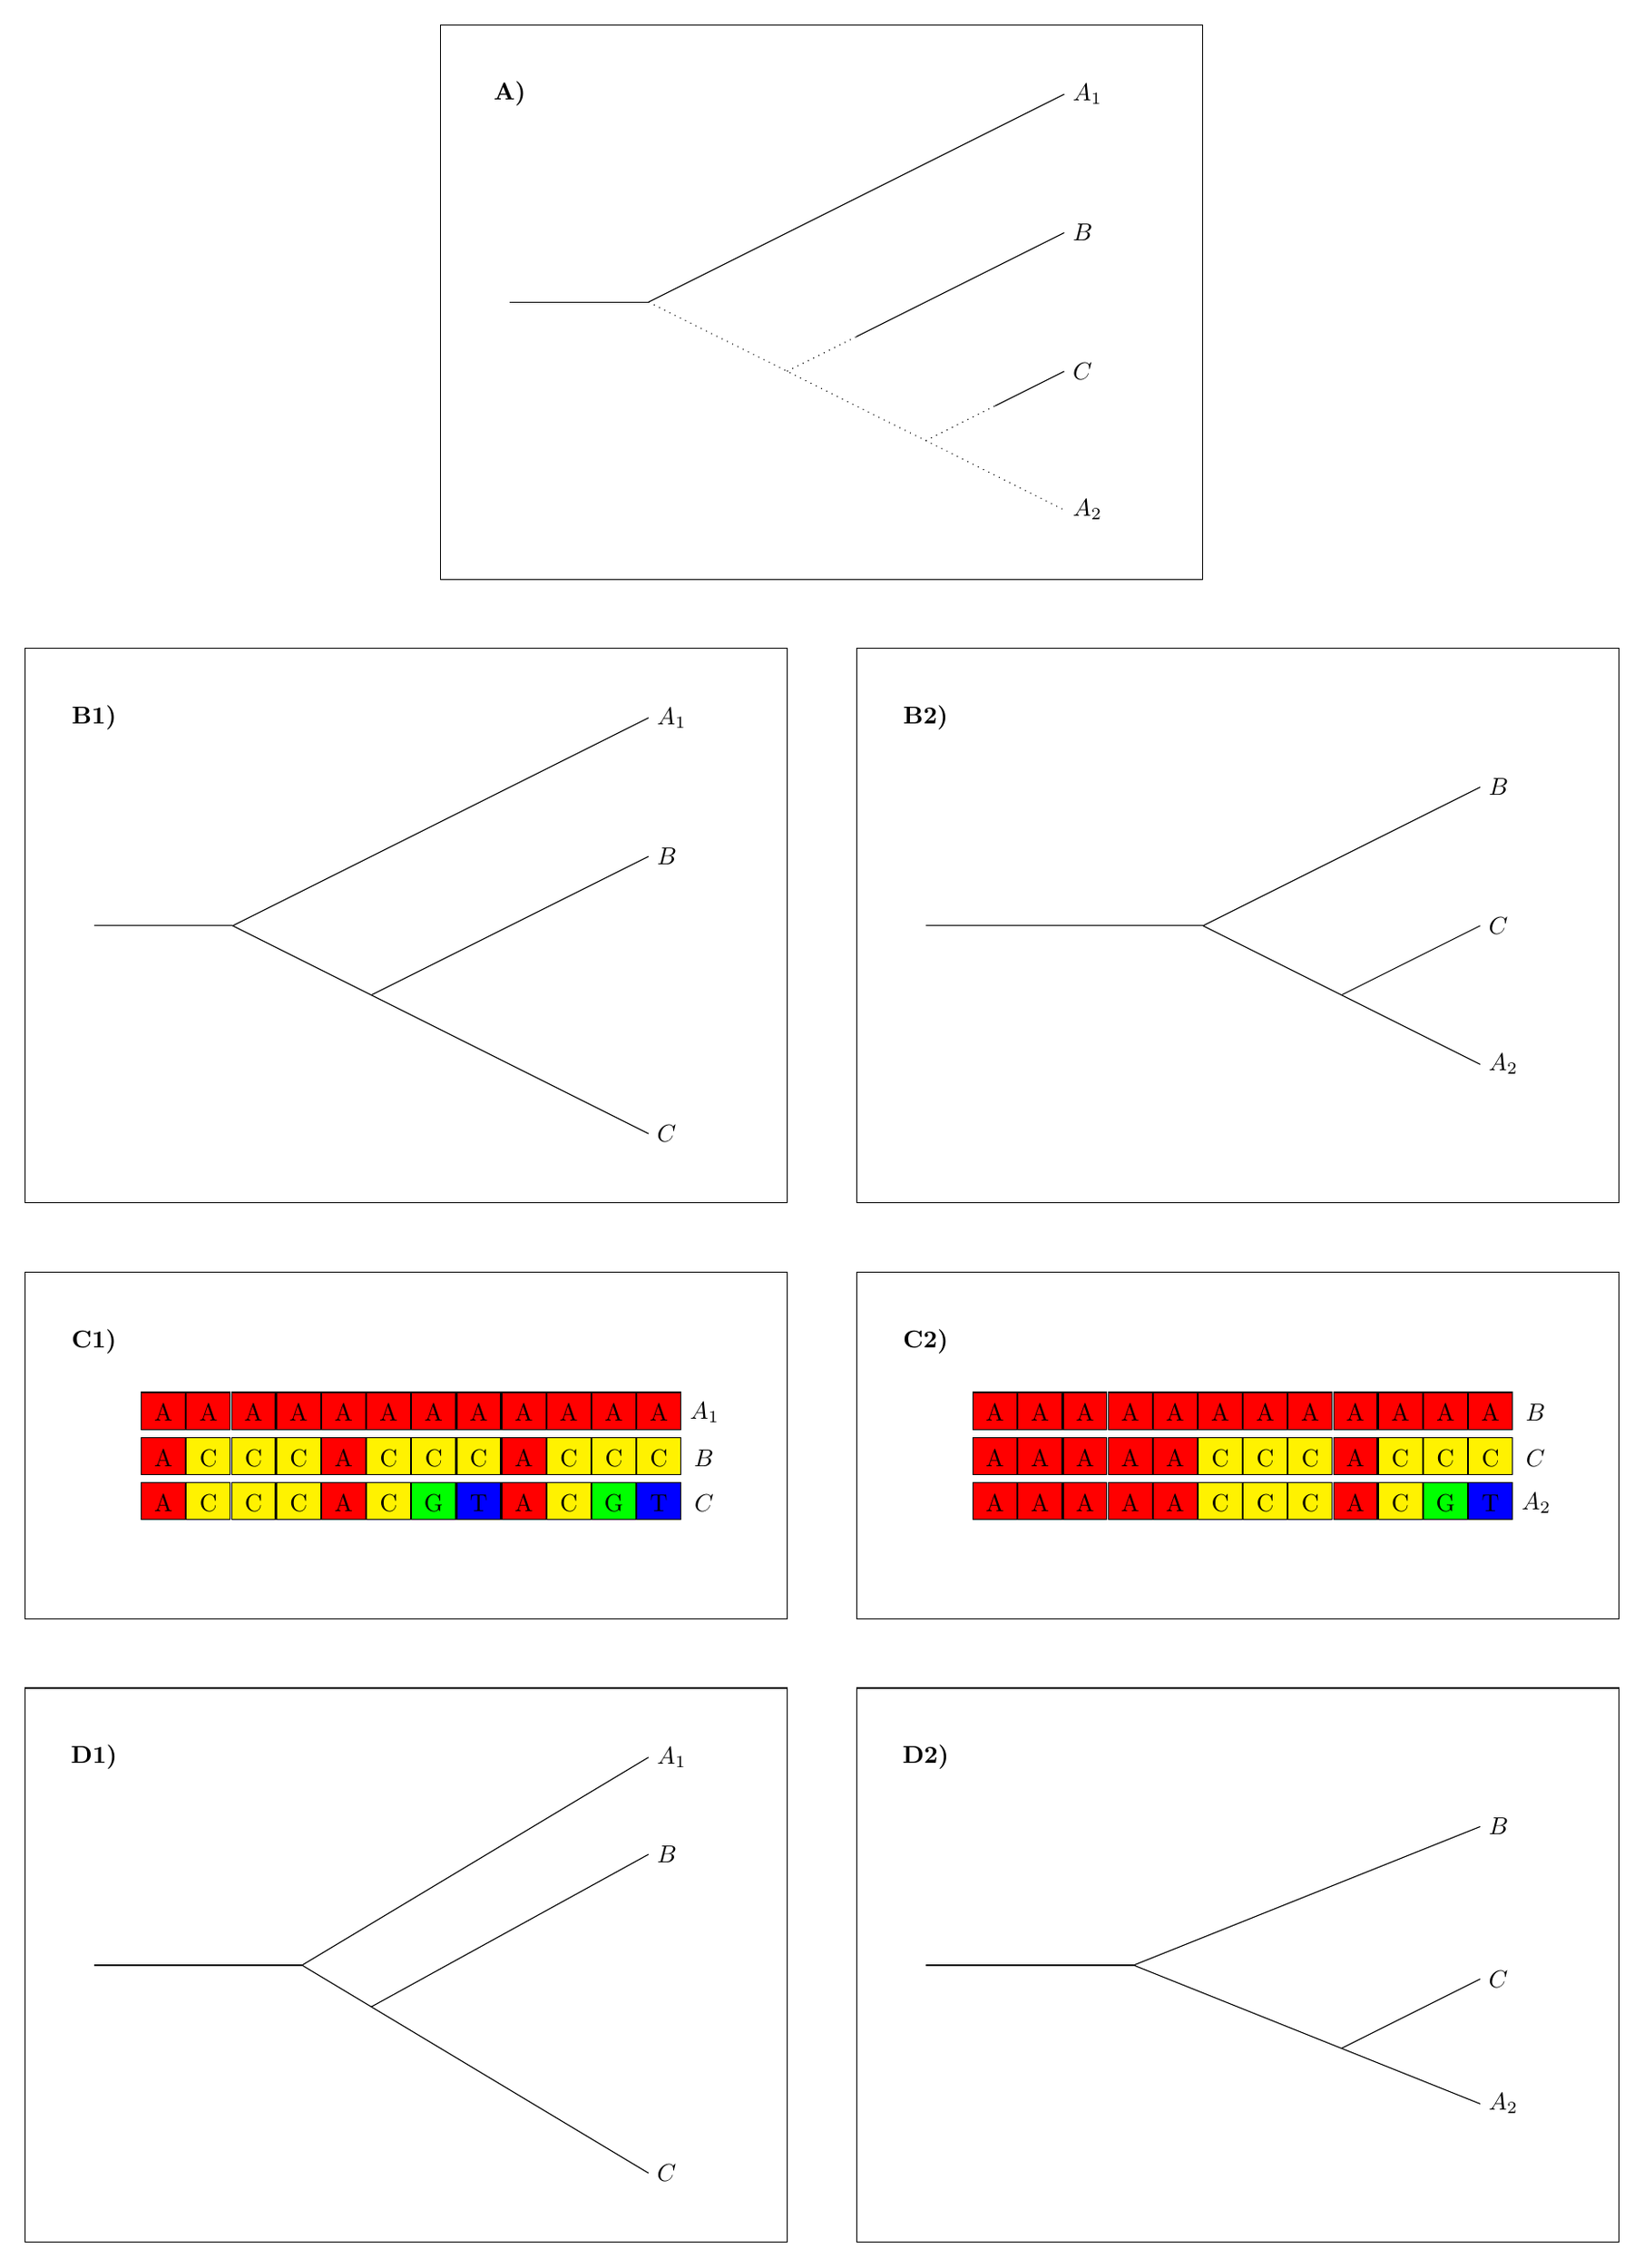
\begin{tikzpicture} 

    % Incipient species tree
    \begin{scope}[shift={(0,0)}] 

      \node[font = \bf] at (0, 0) {A)};
      \draw (-1,1) rectangle (10,-7);

      % Drawing of the phylogeny
      \begin{scope}[shift={(0,-3)}] 
        \draw (0, 0) -- (2,  0); % stem 
        \draw (2, 0) -- (8,  3) node[anchor=west] {$A_1$};
        \draw[dotted] (4,  -1) -- (5, -0.5); \draw (5, -0.5) -- (8, 1) node[anchor=west] {$B$};
        \draw[dotted] (6,  -2) -- (7, -1.5); \draw (7, -1.5) -- (8, -1) node[anchor=west] {$C$};
        \draw[dotted] (2,0) -- (8, -3) node[anchor=west] {$A_2$};
      \end{scope} % Drawing of the phylogeny

    \end{scope}


    % Species tree, oldest
    \begin{scope}[shift={(-6,-9)}] 

      \node[font = \bf] at (0.0, 0  ) {B1)};
      \draw (-1,1) rectangle (10,-7);

      % Drawing of the species tree, oldest
      \begin{scope}[shift={(0,-3)}] 
        \draw (0, 0) -- (2,  0); % stem 
        \draw (2, 0) -- (8,  3) node[anchor=west] {$A_1$};
        \draw (4,  -1) -- (8, 1) node[anchor=west] {$B$};
        \draw (2,0) -- (8, -3) node[anchor=west] {$C$};
      \end{scope} % Drawing of the species tree, oldest

    \end{scope}


    % Species tree, youngest
    \begin{scope}[shift={( 6,-9)}] 

      \node[font = \bf] at (0, 0) {B2)};
      \draw (-1,1) rectangle (10,-7);

      % Drawing of the species tree, youngest
      \begin{scope}[shift={(0,-3)}] 
        \draw (0, 0) -- (4,  0); % stem 
        \draw (4, 0) -- (8,  2) node[anchor=west] {$B$};
        \draw (6,-1) -- (8,  0) node[anchor=west] {$C$};
        \draw (4, 0) -- (8, -2) node[anchor=west] {$A_2$};
      \end{scope} % Drawing of the species tree, youngest

    \end{scope}

    % Alignment, oldest
    \begin{scope}[shift={(-6,-18)}] 

      \node[font = \bf] at (0.0, 0  ) {C1)};
      \draw (-1,1) rectangle (10,-4);

      % Drawing of the alignment
      \begin{scope}[shift={(1,-1)}, text width = 4mm, text height = 3mm, align = center, scale = 1.3] 

        \node[draw, fill = red   ] at (0.0, 0  ) {A};
        \node[draw, fill = red   ] at (0.5, 0  ) {A};
        \node[draw, fill = red   ] at (1.0, 0  ) {A};
        \node[draw, fill = red   ] at (1.5, 0  ) {A};
        \node[draw, fill = red   ] at (2.0, 0  ) {A};
        \node[draw, fill = red   ] at (2.5, 0  ) {A};
        \node[draw, fill = red   ] at (3.0, 0  ) {A};
        \node[draw, fill = red   ] at (3.5, 0  ) {A};
        \node[draw, fill = red   ] at (4.0, 0  ) {A};
        \node[draw, fill = red   ] at (4.5, 0  ) {A};
        \node[draw, fill = red   ] at (5.0, 0  ) {A};
        \node[draw, fill = red   ] at (5.5, 0  ) {A};
        \node[                   ] at (6.0, 0  ) {$A_1$};

        \node[draw, fill = red   ] at (0.0, -0.5) {A};
        \node[draw, fill = yellow] at (0.5, -0.5) {C};
        \node[draw, fill = yellow] at (1.0, -0.5) {C};
        \node[draw, fill = yellow] at (1.5, -0.5) {C};
        \node[draw, fill = red   ] at (2.0, -0.5) {A};
        \node[draw, fill = yellow] at (2.5, -0.5) {C};
        \node[draw, fill = yellow] at (3.0, -0.5) {C};
        \node[draw, fill = yellow] at (3.5, -0.5) {C};
        \node[draw, fill = red   ] at (4.0, -0.5) {A};
        \node[draw, fill = yellow] at (4.5, -0.5) {C};
        \node[draw, fill = yellow] at (5.0, -0.5) {C};
        \node[draw, fill = yellow] at (5.5, -0.5) {C};
        \node[                   ] at (6.0, -0.5) {$B$};

        \node[draw, fill = red] at (0.0, -1.0) {A};
        \node[draw, fill = yellow] at (0.5, -1.0) {C};
        \node[draw, fill = yellow] at (1.0, -1.0) {C};
        \node[draw, fill = yellow] at (1.5, -1.0) {C};
        \node[draw, fill = red   ] at (2.0, -1.0) {A};
        \node[draw, fill = yellow] at (2.5, -1.0) {C};
        \node[draw, fill = green ] at (3.0, -1.0) {G};
        \node[draw, fill = blue  ] at (3.5, -1.0) {T};
        \node[draw, fill = red   ] at (4.0, -1.0) {A};
        \node[draw, fill = yellow] at (4.5, -1.0) {C};
        \node[draw, fill = green ] at (5.0, -1.0) {G};
        \node[draw, fill = blue  ] at (5.5, -1.0) {T};
        \node[                   ] at (6.0, -1.0) {$C$};

      \end{scope} % Drawing of the alignment

    \end{scope}

    % Alignment, youngest
    \begin{scope}[shift={(6,-18)}] 

      \node[font = \bf] at (0.0, 0  ) {C2)};
      \draw (-1,1) rectangle (10,-4);

      % Drawing of the alignment
      \begin{scope}[shift={(1,-1)}, text width = 4mm, text height = 3mm, align = center, scale = 1.3] 

        \node[draw, fill = red   ] at (0.0, 0  ) {A};
        \node[draw, fill = red   ] at (0.5, 0  ) {A};
        \node[draw, fill = red   ] at (1.0, 0  ) {A};
        \node[draw, fill = red   ] at (1.5, 0  ) {A};
        \node[draw, fill = red   ] at (2.0, 0  ) {A};
        \node[draw, fill = red   ] at (2.5, 0  ) {A};
        \node[draw, fill = red   ] at (3.0, 0  ) {A};
        \node[draw, fill = red   ] at (3.5, 0  ) {A};
        \node[draw, fill = red   ] at (4.0, 0  ) {A};
        \node[draw, fill = red   ] at (4.5, 0  ) {A};
        \node[draw, fill = red   ] at (5.0, 0  ) {A};
        \node[draw, fill = red   ] at (5.5, 0  ) {A};
        \node[                   ] at (6.0, 0  ) {$B$};

        \node[draw, fill = red   ] at (0.0, -0.5) {A};
        \node[draw, fill = red   ] at (0.5, -0.5) {A};
        \node[draw, fill = red   ] at (1.0, -0.5) {A};
        \node[draw, fill = red   ] at (1.5, -0.5) {A};
        \node[draw, fill = red   ] at (2.0, -0.5) {A};
        \node[draw, fill = yellow] at (2.5, -0.5) {C};
        \node[draw, fill = yellow] at (3.0, -0.5) {C};
        \node[draw, fill = yellow] at (3.5, -0.5) {C};
        \node[draw, fill = red   ] at (4.0, -0.5) {A};
        \node[draw, fill = yellow] at (4.5, -0.5) {C};
        \node[draw, fill = yellow] at (5.0, -0.5) {C};
        \node[draw, fill = yellow] at (5.5, -0.5) {C};
        \node[                   ] at (6.0, -0.5) {$C$};

        \node[draw, fill = red   ] at (0.0, -1.0) {A};
        \node[draw, fill = red   ] at (0.5, -1.0) {A};
        \node[draw, fill = red   ] at (1.0, -1.0) {A};
        \node[draw, fill = red   ] at (1.5, -1.0) {A};
        \node[draw, fill = red   ] at (2.0, -1.0) {A};
        \node[draw, fill = yellow] at (2.5, -1.0) {C};
        \node[draw, fill = yellow] at (3.0, -1.0) {C};
        \node[draw, fill = yellow] at (3.5, -1.0) {C};
        \node[draw, fill = red   ] at (4.0, -1.0) {A};
        \node[draw, fill = yellow] at (4.5, -1.0) {C};
        \node[draw, fill = green ] at (5.0, -1.0) {G};
        \node[draw, fill = blue  ] at (5.5, -1.0) {T};
        \node[                   ] at (6.0, -1.0) {$A_2$};

      \end{scope} % Drawing of the alignment

    \end{scope}



    % Estimated species tree, oldest
    \begin{scope}[shift={(-6,-24)}] 

      \node[font = \bf] at (0, 0) {D1)};
      \draw (-1,1) rectangle (10,-7);

      \begin{scope}[shift={(0,-3)}] 
        \draw (0, 0) -- (3,  0);
        \draw (3, 0) -- (8, 3) node[anchor=west] {$A_1$};
        \draw (4,-0.6) -- (8, 1.6) node[anchor=west] {$B$};
        \draw (3, 0) -- (8,-3) node[anchor=west] {$C$};
      \end{scope}

    \end{scope}


    % Estimated species tree, youngest
    \begin{scope}[shift={(6,-24)}] 

      \node[font = \bf] at (0, 0) {D2)};
      \draw (-1,1) rectangle (10,-7);

      \begin{scope}[shift={(0,-3)}] 
        \draw (0, 0) -- (3,  0);
        \draw (3, 0) -- (8,  2) node[anchor=west] {$B$};
        \draw (6,-1.2) -- (8, -0.2) node[anchor=west] {$C$};
        \draw (3, 0) -- (8, -2) node[anchor=west] {$A_2$};
      \end{scope}

    \end{scope}

  \end{tikzpicture}
} % End of create_figure_experiment definition
%%%%%%%%%%%%%%%%%%%%%%%%%%%%%%%%%%%%%%%%%%%%%%%%%%%%%%%%%%%%%%%%%%%%%%%%%%%%%%%%




%%%%%%%%%%%%%%%%%%%%%%%%%%%%%%%%%%%%%%%%%%%%%%%%%%%%%%%%%%%%%%%%%%%%%%%%%%%%%%%%
% Create the TikZ picture of fig:sampling
%%%%%%%%%%%%%%%%%%%%%%%%%%%%%%%%%%%%%%%%%%%%%%%%%%%%%%%%%%%%%%%%%%%%%%%%%%%%%%%%
\newcommand{\CreateTikzFigureSampling} {

  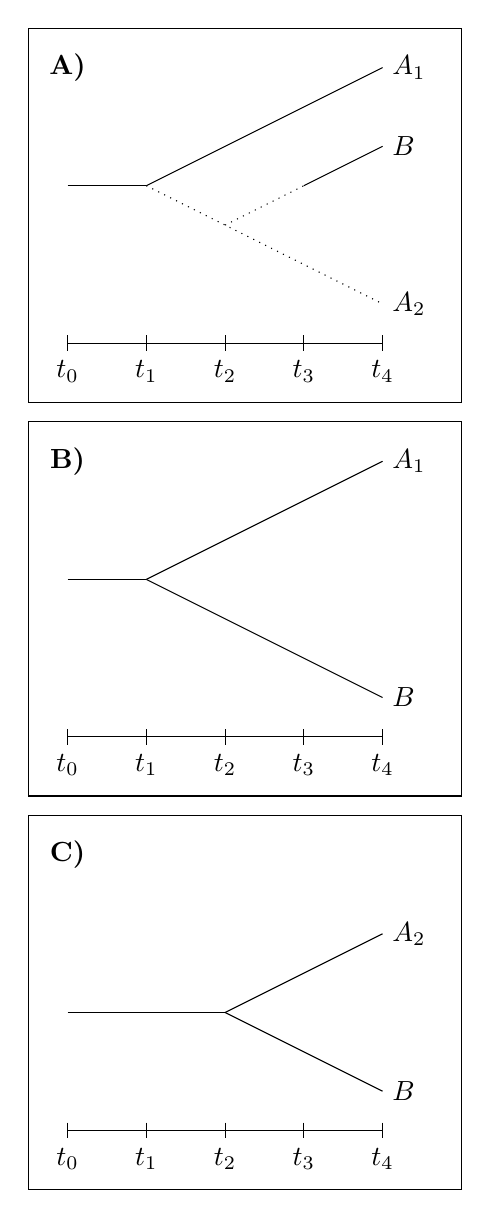
\begin{tikzpicture}[scale = 0.5] 

    \begin{scope}[shift={(0,0)}] 

      \node[font = \bf] at (0, 0) {A)};
      \draw (-1,1) rectangle (10,-8.5);

      % Drawing of the phylogeny
      \begin{scope}[shift={(0,-3)}] 
        \draw (0, 0) -- (2,  0);
        \draw (2, 0) -- (8,  3) node[anchor=west] {$A_1$};
        \draw[dotted] (2, 0) -- (8, -3) node[anchor=west] {$A_2$};
        \draw[dotted] (4, -1) -- (6, 0);
        \draw (6, 0) -- (8, 1) node[anchor=west] {$B$};
        % time scale
        \draw (0, -4) -- (8,  -4);
        \draw (0, -3.8) -- (0,  -4.2) node[anchor=north] {$t_0$};
        \draw (2, -3.8) -- (2,  -4.2) node[anchor=north] {$t_1$};
        \draw (4, -3.8) -- (4,  -4.2) node[anchor=north] {$t_2$};
        \draw (6, -3.8) -- (6,  -4.2) node[anchor=north] {$t_3$};
        \draw (8, -3.8) -- (8,  -4.2) node[anchor=north] {$t_4$};
      \end{scope} % Drawing of the phylogeny

    \end{scope}
    \begin{scope}[shift={(0, -10)}] 

      \node[font = \bf] at (0, 0) {B)};
      \draw (-1,1) rectangle (10,-8.5);

      % Drawing of the phylogeny
      \begin{scope}[shift={(0,-3)}] 
        \draw (0, 0) -- (2,  0);
        \draw (2, 0) -- (8,  3) node[anchor=west] {$A_1$};
        \draw (2, 0) -- (8, -3) node[anchor=west] {$B$};
        % time scale
        \draw (0, -4) -- (8,  -4);
        \draw (0, -3.8) -- (0,  -4.2) node[anchor=north] {$t_0$};
        \draw (2, -3.8) -- (2,  -4.2) node[anchor=north] {$t_1$};
        \draw (4, -3.8) -- (4,  -4.2) node[anchor=north] {$t_2$};
        \draw (6, -3.8) -- (6,  -4.2) node[anchor=north] {$t_3$};
        \draw (8, -3.8) -- (8,  -4.2) node[anchor=north] {$t_4$};
      \end{scope} % Drawing of the phylogeny

    \end{scope}
    \begin{scope}[shift={(0,-20)}] 

      \node[font = \bf] at (0, 0) {C)};
      \draw (-1,1) rectangle (10,-8.5);

      % Drawing of the phylogeny
      \begin{scope}[shift={(0,-3)}] 
        \draw (0, -1) -- (4, -1) ;
        \draw (4, -1) -- (8, -3) node[anchor=west] {$B$};
        \draw (4, -1) -- (8,  1) node[anchor=west] {$A_2$};
        % time scale
        \draw (0, -4) -- (8,  -4);
        \draw (0, -3.8) -- (0,  -4.2) node[anchor=north] {$t_0$};
        \draw (2, -3.8) -- (2,  -4.2) node[anchor=north] {$t_1$};
        \draw (4, -3.8) -- (4,  -4.2) node[anchor=north] {$t_2$};
        \draw (6, -3.8) -- (6,  -4.2) node[anchor=north] {$t_3$};
        \draw (8, -3.8) -- (8,  -4.2) node[anchor=north] {$t_4$};
      \end{scope} % Drawing of the phylogeny

    \end{scope}
  \end{tikzpicture}

} % End of create_figure_experiment definition
%%%%%%%%%%%%%%%%%%%%%%%%%%%%%%%%%%%%%%%%%%%%%%%%%%%%%%%%%%%%%%%%%%%%%%%%%%%%%%%%



% Use double spacing
\usepackage{setspace}
\doublespacing

\usepackage{listings}
\usepackage{hyperref}
\usepackage{todonotes}
\usepackage{verbatim}
\usepackage{pgf}
\usepackage{bm}

% TikZ and friends
\usepackage{tikz}
\usepackage{tkz-graph}
\usepackage{pgf}
\usetikzlibrary{arrows,automata}

% Style of listings
% From http://r.789695.n4.nabble.com/How-to-nicely-display-R-code-with-the-LaTeX-package-listings-tp4648110.html
\usepackage{fancyvrb} 
\definecolor{codegreen}{rgb}{0,0.6,0}
\definecolor{codegray}{rgb}{0.5,0.5,0.5}
\definecolor{codepurple}{rgb}{0.58,0,0.82}
\definecolor{backcolor}{rgb}{0.95,0.95,0.92}
\lstdefinestyle{mystyle}{
  language=R,% set programming language
  basicstyle=\ttfamily\small,% basic font style
  commentstyle=\color{gray},% comment style
  % numbers=left,% display line numbers on the left side
  numberstyle=\scriptsize,% use small line numbers
  numbersep=10pt,% space between line numbers and code
  tabsize=2,% sizes of tabs
  showstringspaces=false,% do not replace spaces in strings by a certain character
  captionpos=b,% positioning of the caption below
  breaklines=true,% automatic line breaking
  escapeinside={(*}{*)},% escaping to LaTeX
  fancyvrb=true,% verbatim code is typset by listings
  extendedchars=false,% prohibit extended chars (chars of codes 128--255)
  alsoletter={.<-},% becomes a letter
  alsoother={$},% becomes other
  otherkeywords={!=, ~, $, \&, \%/\%, \%*\%, \%\%, <-, <<-, /},% other keywords
  deletekeywords={c}% remove keywords 
}
\lstset{style=mystyle}

% Adds numbered lines
\usepackage{lineno}
\linenumbers

% Use TODO notes
\usepackage{todonotes}


% Rename 'Abstract' to 'Summary 
\usepackage[english]{babel}
\addto{\captionsenglish}{\renewcommand{\abstractname}{Summary}}

\begin{document}

\maketitle

%%%%%%%%%%%%%%%%%%%%%%%%%%%%%%%%%%%%%%%%%%%%%%%%%%%%%%%%%%%%%%%%%%%%%%%%%%%%%%%%%%%%%%
\section{Introduction}
%%%%%%%%%%%%%%%%%%%%%%%%%%%%%%%%%%%%%%%%%%%%%%%%%%%%%%%%%%%%%%%%%%%%%%%%%%%%%%%%%%%%%%

Phylogenetics enables us to infer which species lived when and
estimate how long it took for a species to give rise to a new
lineage. Phylogenies show us taxa that have completed speciation, yet
those taxa only: species that are in the process of speciation are 
overlooked.

There are multiple reasons why a speciation event, during
or after its course, goes unnoticed. It may be that the build-up
of reproductive isolation is still in an intermediate stage. But it
may also be that speciation has completed, but we, humans, have not
yet observed it. One example are the four African giraffe species, 
that have been thought to have been one single species up until 2016,
where the MRCA of the two most recent species goes back 1.6 million years.

It took some time until the Birth-Death model, a phylogenetic model
assuming constant rates of speciation and extinction, got extended
by a version that incorporates the fact that speciation takes time.
This extension is called the Protracted Birth-Death model. In this
model, a branching event does not give rise to a new species, but to
a new species-to-be, called an incipient species. Such an incipient
species may go extinct, or finish its speciation to become a good species.

Although we know speciation takes time, most of our theoretical 
phylogenetic modeling ignores this fact. To the best of our knowledge,
there is no tool incorporating this fact. One reason may be to ease
computation, enabling researchers to work on bigger phylogenies (with
more power statistical power) instead. Additionally, speciation being
protracted is only playing a role in the present. As seen from the present,
all older species have finished speciation, as we -by definition- recognize
these species as such. 

There are problems with ignoring protracted speciation. A very pragmatic
example is the conservation of the now four smaller groups of giraffes,
instead of one big group. But from a more theoretical perspective, the
observed decline of speciation rate in time (excluding the contemporary human-driven
mass extinction event) may be explained by these new species not being 
recognized yet. Another problem is that the MRCA of young species is estimated 
incorrectly, as in the BD model a species can be ultra-young (as speciation
is assumed to be instantaneous), where the PBD model will place these MRCAs
further back in time (as two events need to have finished completion).

From a theoretical point of view, there is another reason why protracted
speciation has yet become a member of our toolbox: there is no framework
where it fits in: a framework assumes either an analysis at the species or
subspecies level. When picking a tool that does its analysis at the
species level, there is no protocol how to select which incipient species
gets to represent the full species it is still a member of. When picking
a tool at the sub-species level, the incipient state disappears as a
sub-species lineage, and the process degrades to an ordinary birth-death 
process.

This research's goals are two-fold, which are (1) to quantify the
inference error we make with contemporary tools assuming a Birth-Death
process, and (2) to establish a protocol how to sample incipient species
to represent a species in such a tool.

To quantify the inference error, we simulate 'true' incipient species
trees, sample a 'true' species trees from those, simulate a DNA alignments 
that follows a species tree's ontogeny, then infer a posterior of
phylogenies from each alignment. The 'true' species tree is compared to
the posterior's phylogenies with the nLTT statistic, which can be viewed
as a measure of similarity. We expect this error to increase with an
increasing protractednedness (that is, a low speciation completion rate),
but as the extent of this error has never been measured, we will be the
first to measure it.

To establish a protocol how to sample incipient species to represent species,
we compare two sampling methods that are opposites of one another: one
method is to select the oldest sub-species member to represent a species,
the other method picks the youngest sub-species member. As we do not have
a way to determine which sampling method will be better, all we determine
is if the sampling methods are different. We expect these
sampling methods to be equivalent. This research measures the extent to
which this is true.

This exploratorary research will produce a data set that maps the biological
parameters to the error made. The data set will consist out of two files:
one containing raw data, the other summarized data. 
A data file should be convenient to handle, thus as an upper limit for this data set's size, 
we use the maximum size of a table (called a data frame) of the R programming 
language. Within R, such a table may have maximally $2^{32}-1$ cells and occupy
less then 2 gigabytes in memory. 
The raw data file will contain parameters and 1000 nLTT statistics values.
Each row will contain the parameter set and these nLTT statistics.
From the constraints of the R programming language, this allows for 40K rows. 
The file with the summarized data will provide summary statistics of the raw
data. Each row will contain a parameter set, summary statistics and other
measurements. See the appendix, chapter 'Data set specifications', for the full list.

%%%%%%%%%%%%%%%%%%%%%%%%%%%%%%%%%%%%%%%%%%%%%%%%%%%%%%%%%%%%%%%%%%%%%%%%%%%%%%%%
\section{Methods}
%%%%%%%%%%%%%%%%%%%%%%%%%%%%%%%%%%%%%%%%%%%%%%%%%%%%%%%%%%%%%%%%%%%%%%%%%%%%%%%%

We simulate protracted birth-death trees. In a protracted birth-death tree,
species-to-be are present, but not yet recognized as different from
their ancestral species. We simulate these trees from the biological parameters 
in a factorial fashion. Excluded from this are combinations of parameters in which
speciation initiation rate is lower or equal the extinction rate, as these
are biologically irrelevant. Out of computational necessity, 
parameter combinations that result in an expected number of taxa above 1000 
are removed as well.

From these PBD trees, we sample species tree in two different ways. 
From all incipient species-to-be, we pick either the youngest or oldest
species-to-be to represent the full species. This species tree we refer
to as 'the true species tree'.

From a species tree, we simulate a DNA alignment that has the same history
as the phylogeny. The nucleotides of the DNA alignment follow a JC69
nucleotide substitution model, in which all nucleotide-to-nucleotide transitions
are equally likely. Although this may seem as a simplification, in our Bayesian
inference we can use this as a prior, which we know is the truth.

The DNA sequence length and mutation rate was chosen as such to provide one
nucleotide change per 1000 years per lineage. As our time unit is in 
millions of years, this equates to a rate of 1000 nucleotide substitutions 
changes per time unit per lineage. To provide for each substitution being unique,
we simulate as much DNA nucleotides as expected mutations, which equals the
nucleotide substitution rate times the crown age, which equals 15K. As this
mutation rate is constant over all branches, it in effect follows a strict 
clock model.

The simulated alignment is the data that could be measured in the field.
This alignment is used to infer a posterior of, using BEAST2. We assume a
JC69 nucleotide substitution (as we do use that), a strict clock model (as
we have that) and a Birth-Death tree prior (as this simplification is the goal
of this research). Additionally, we assume a MRCA prior with a normal distribution
with a mean of the crown age, and a standard deviation of 0.001 time units. 0.001
time units equates to 1000 years, which is the same resolution as which the
alignment is created. After discarding a burn-in of 10\%, the MCMC algorithm must 
result in an ESS of the posterior of at least 200 and the MCMC chain length is 
chosen as such that this is the case for all simulations. For simulations
with an ESS below 200, their MCMC chain length is elongated. An
MCMC chain is elongated by the proportion that is expected to increase it to 220. 
For example, would an ESS be 165, increasing its MCMC chain length by 33\% 
would bring it to (165\%*1.33=) 220. We use
220 as a safeguard to prevent an asymptotic approach to 200. 

The nLTT statistic is used to quantify the similarity of each posterior's phylogeny 
with 'the true species tree'. In this way, a distribution of phylogenies
is transformed to a distribution of nLTT statistics. With this, the generative
model of this experiment has been completely described, from parameter estimates
to data (nLTT statistics) generated.

To quantify the effect of sampling (either the youngest or oldest species-to-be to represent
a species), for each parameter set that allows for incipient species,
we simulate 1000 incipient species trees that result in different species trees
when sampled either way. From each species tree, we compare the nLTT distributions
for the two sampling methods. These distributions are compared 
using the method described in [Kruschke 2013], with a non-informative
prior. In brief: if the 95\% Highest Density Interval of the differences between 
these two distributions excludes zero, it is credible the distributions are different. 

To measure if protractedness matters, we compare the nLTT distribution per
combination of speciation initiation and extinction rate for a protracted
setting with its non-protracted (with a high speciation completion 
rate) setting. So, for each speciation initiation and extinction rate, 
the nLTT statistic distribution of the 
non-protracted setting is used as the baseline. That distribution is compared
with each protracted setting. This is done the same way as with the two
different sampling methods. [NOTE: we expect nLTT to go up for increasing SCR,
this should be in the method].

[NOTE: We do have more info, from Rampal's earlier articles. Perhaps this 
info can be put in]

[NOTE: as we know the expected number of lineages through time for both BD and PBD
model, we expect it to fall with the 95\% Highest Density Interval. It would also
increase support for Rampal's choice of parameter values (next to their 
computational feasability)]

%%%%%%%%%%%%%%%%%%%%%%%%%%%%%%%%%%%%%%%%%%%%%%%%%%%%%%%%%%%%%%%%%%%%%%%%%%%%%%%%%%%%%%
\section{Results}
%%%%%%%%%%%%%%%%%%%%%%%%%%%%%%%%%%%%%%%%%%%%%%%%%%%%%%%%%%%%%%%%%%%%%%%%%%%%%%%%%%%%%%

\begin{figure}[]
  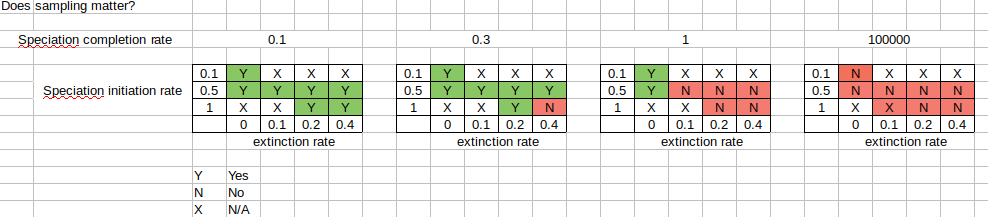
\includegraphics[width=0.9\textwidth]{fig_does_sampling_matter.png}
\end{figure}

\begin{figure}[]
  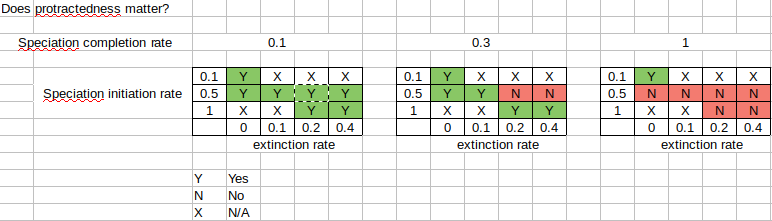
\includegraphics[width=0.9\textwidth]{fig_does_protractedness_matter.png}
\end{figure}

%%%%%%%%%%%%%%%%%%%%%%%%%%%%%%%%%%%%%%%%%%%%%%%%%%%%%%%%%%%%%%%%%%%%%%%%%%%%%%%%%%%%%%
\section{Discussion}
%%%%%%%%%%%%%%%%%%%%%%%%%%%%%%%%%%%%%%%%%%%%%%%%%%%%%%%%%%%%%%%%%%%%%%%%%%%%%%%%%%%%%%


%%%%%%%%%%%%%%%%%%%%%%%%%%%%%%%%%%%%%%%%%%%%%%%%%%%%%%%%%%%%%%%%%%%%%%%%%%%%%%%%%%%%%%
\section{Acknowledgements}
%%%%%%%%%%%%%%%%%%%%%%%%%%%%%%%%%%%%%%%%%%%%%%%%%%%%%%%%%%%%%%%%%%%%%%%%%%%%%%%%%%%%%%

We would like to thank the Center for Information Technology of the University of Groningen for their support
and for providing access to the Peregrine high performance computing cluster.

%%%%%%%%%%%%%%%%%%%%%%%%%%%%%%%%%%%%%%%%%%%%%%%%%%%%%%%%%%%%%%%%%%%%%%%%%%%%%%%%%%%%%%
\section{Authors' contributions}
%%%%%%%%%%%%%%%%%%%%%%%%%%%%%%%%%%%%%%%%%%%%%%%%%%%%%%%%%%%%%%%%%%%%%%%%%%%%%%%%%%%%%%

%%%%%%%%%%%%%%%%%%%%%%%%%%%%%%%%%%%%%%%%%%%%%%%%%%%%%%%%%%%%%%%%%%%%%%%%%%%%%%%%%%%%%%
% Bibliography
%%%%%%%%%%%%%%%%%%%%%%%%%%%%%%%%%%%%%%%%%%%%%%%%%%%%%%%%%%%%%%%%%%%%%%%%%%%%%%%%%%%%%%
% MEE style
\bibliographystyle{mee}
\bibliography{article}
%%%%%%%%%%%%%%%%%%%%%%%%%%%%%%%%%%%%%%%%%%%%%%%%%%%%%%%%%%%%%%%%%%%%%%%%%%%%%%%%%%%%%%

%%%%%%%%%%%%%%%%%%%%%%%%%%%%%%%%%%%%%%%%%%%%%%%%%%%%%%%%%%%%%%%%%%%%%%%%%%%%%%%%%%%%%%
\appendix
%%%%%%%%%%%%%%%%%%%%%%%%%%%%%%%%%%%%%%%%%%%%%%%%%%%%%%%%%%%%%%%%%%%%%%%%%%%%%%%%%%%%%%

%%%%%%%%%%%%%%%%%%%%%%%%%%%%%%%%%%%%%%%%%%%%%%%%%%%%%%%%%%%%%%%%%%%%%%%%%%%%%%%%%%%%%%
\section{Data set specifications}
%%%%%%%%%%%%%%%%%%%%%%%%%%%%%%%%%%%%%%%%%%%%%%%%%%%%%%%%%%%%%%%%%%%%%%%%%%%%%%%%%%%%%%

The raw data file will consist of 40K rows. On each row there will be 1012 values:

\begin{itemize}  
  \item 12 simulation parameters:
  \begin{enumerate}  
    \item speciation initiation rate
    \item speciation completion rate
    \item extinction rate
    \item crown age
    \item crown age sigma
    \item sampling method
    \item mutation rate
    \item sequence length
    \item mcmc length
    \item tree sim rng seed
    \item alignment rng seed
    \item beast2 rnd seed
  \end{enumerate}
  \item 1000 nLTT statistics
\end{itemize}

The summarized data file will consist of 40K rows. On each row there will be 29 values:

\begin{itemize}  
  \item 12 simulation parameters:
  \begin{enumerate}  
    \item speciation initiation rate
    \item speciation completion rate
    \item extinction rate
    \item crown age
    \item crown age sigma
    \item sampling method
    \item mutation rate
    \item sequence length
    \item mcmc length
    \item tree sim rng seed
    \item alignment rng seed
    \item beast2 rnd seed
  \end{enumerate}
  \item number of taxa in incipient species tree (also: number of subspecies)
  \item number of taxa in species tree (also: number of species)
  \item mean nLTT statistic
  \item median nLTT statistic
  \item lower bound of 95\% HPD value of nLTT statistic
  \item upper bound of 95\% HPD value of nLTT statistic
  \item 11 ESSes of all parameters estimated by BEAST2:
  \begin{enumerate}  
    \item posterior
    \item likelihood 
    \item prior 
    \item treeLikelihood 
    \item TreeHeight 
    \item BirthDeath 
    \item BDBirthRate 
    \item BDDeathRate 
    \item logP.mrca 
    \item mrcatime 
    \item clockRate
  \end{enumerate}
\end{itemize}

\end{document}
